\documentclass[12pt,border=0pt]{standalone}

\usepackage[utf8]{inputenc} 
\usepackage{amssymb,amsmath}
\usepackage{tikz}

\usepackage{nicefrac}
\usepackage{youngtab}


\thispagestyle{empty}

\begin{document}

\Yboxdim11pt
\Ylinethick{0.6pt}


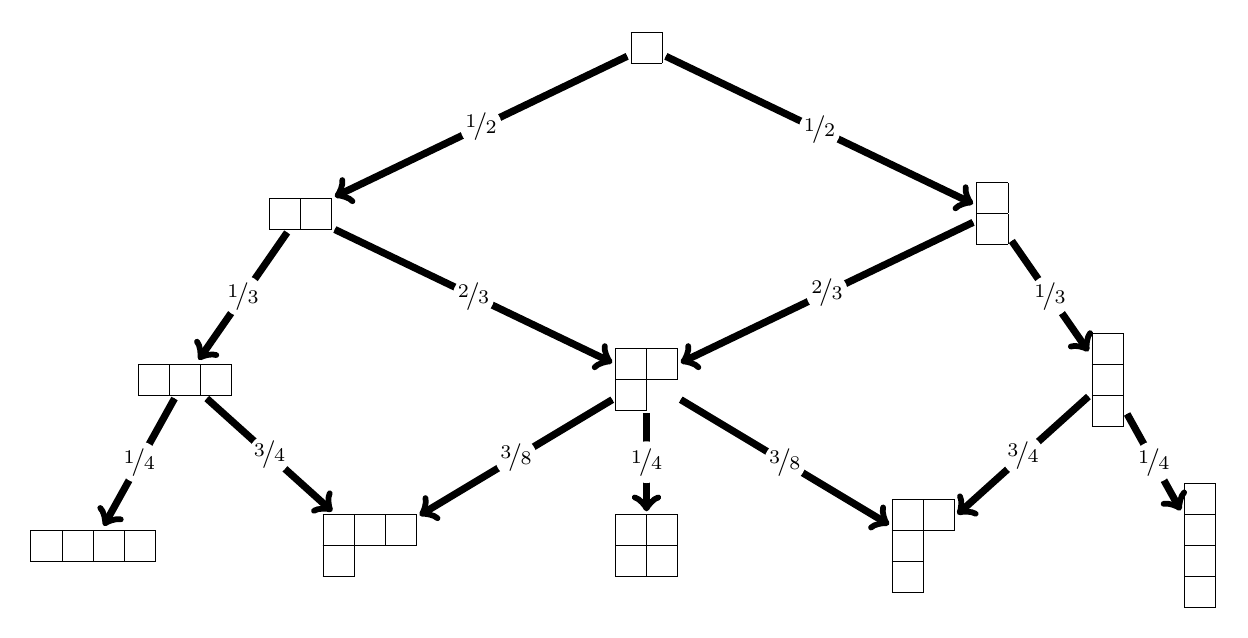
\begin{tikzpicture}[x=10pt,y=6pt]
  \centering
  \tikzset{VertexStyle/.style = {
    shape         = rectangle,
    draw          = none, 
    fill          = white, 
  	line width    = 1pt, 
    text          = black,
    inner sep     = 1pt,
    outer sep     = 0pt,
    minimum size  = 14 pt,
    scale         = 1
    }
  }
  \tikzset{EdgeStyle/.style = {
    draw            = black, 
    thick,
    double          = black,
    double distance = 1pt,
    style = ->
    }
  }
  \tikzset{EdgeLabelStyle/.style = {
    draw          = none,
  	shape         = circle, 
  	line width    = 1pt, 
  	minimum size  = 10pt, 
    inner sep     = 0pt,
    outer sep     = 0pt,
    fill          = white,
    text          = black,
    scale         = 1
    }
  }

	\node[VertexStyle](A1) at (25, 45) {$\yng(1)$};
	\node[VertexStyle](B1) at (12.5, 35) {$\yng(2)$};
	\node[VertexStyle](B2) at (37.5, 35) {$\yng(1,1)$};
	\node[VertexStyle](C1) at (8.33333333333333, 25) {$\yng(3)$};
	\node[VertexStyle](C2) at (25, 25) {$\yng(2,1)$};
	\node[VertexStyle](C3) at (41.6666666666667, 25) {$\yng(1,1,1)$};
	\node[VertexStyle](D1) at (5, 15) {$\yng(4)$};
	\node[VertexStyle](D2) at (15, 15) {$\yng(3,1)$};
	\node[VertexStyle](D3) at (25, 15) {$\yng(2,2)$};
	\node[VertexStyle](D4) at (35, 15) {$\yng(2,1,1)$};
	\node[VertexStyle](D5) at (45, 15) {$\yng(1,1,1,1)$};
	% \node[VertexStyle](E1) at (3.57142857142857, 5) {$\yng(5)$};
	% \node[VertexStyle](E2) at (10.7142857142857, 5) {$\yng(4,1)$};
	% \node[VertexStyle](E3) at (17.8571428571429, 5) {$\yng(3,2)$};
	% \node[VertexStyle](E4) at (25, 5) {$\yng(3,1,1)$};
	% \node[VertexStyle](E5) at (32.1428571428571, 5) {$\yng(2,2,1)$};
	% \node[VertexStyle](E6) at (39.2857142857143, 5) {$\yng(2,1,1,1)$};
	% \node[VertexStyle](E7) at (46.4285714285714, 5) {$\yng(1,1,1,1,1)$};
	\draw[EdgeStyle](A1) to node[EdgeLabelStyle]{$\nicefrac{1}{2}$} (B1);
	\draw[EdgeStyle](A1) to node[EdgeLabelStyle]{$\nicefrac{1}{2}$} (B2);
	\draw[EdgeStyle](B1) to node[EdgeLabelStyle]{$\nicefrac{1}{3}$} (C1);
	\draw[EdgeStyle](B1) to node[EdgeLabelStyle]{$\nicefrac{2}{3}$} (C2);
	\draw[EdgeStyle](B2) to node[EdgeLabelStyle]{$\nicefrac{2}{3}$} (C2);
	\draw[EdgeStyle](B2) to node[EdgeLabelStyle]{$\nicefrac{1}{3}$} (C3);
	\draw[EdgeStyle](C1) to node[EdgeLabelStyle]{$\nicefrac{1}{4}$} (D1);
	\draw[EdgeStyle](C1) to node[EdgeLabelStyle]{$\nicefrac{3}{4}$} (D2);
	\draw[EdgeStyle](C2) to node[EdgeLabelStyle]{$\nicefrac{3}{8}$} (D2);
	\draw[EdgeStyle](C2) to node[EdgeLabelStyle]{$\nicefrac{1}{4}$} (D3);
	\draw[EdgeStyle](C2) to node[EdgeLabelStyle]{$\nicefrac{3}{8}$} (D4);
	\draw[EdgeStyle](C3) to node[EdgeLabelStyle]{$\nicefrac{3}{4}$} (D4);
	\draw[EdgeStyle](C3) to node[EdgeLabelStyle]{$\nicefrac{1}{4}$} (D5);

  \end{tikzpicture}

\end{document}
